\documentclass[11pt,a4paper]{article}
\usepackage[margin=2.6cm]{geometry}
\usepackage{graphicx}
\usepackage{amsmath}
\usepackage{booktabs}
\usepackage{microtype}
\usepackage[hidelinks]{hyperref}
\usepackage{caption}
\captionsetup{font=small,labelfont=bf,width=0.92\textwidth}
\usepackage{abstract}
\setlength{\parskip}{2pt}

\title{\textbf{The Fractal as a Shared Dictionary:\\
Lossless Compression of Small Payloads\\
via a Regenerable Mandelbrot Codebook}}
\author{Wietse Stienstra\thanks{Concept and architecture: the fractal number-registry
and ``store the \emph{where}, not the \emph{what}'' scheme this paper implements.}
\and Patrick (Claude, Anthropic)\thanks{Implementation, experiments, and manuscript.
All results roundtrip-verified; code and benchmark harness available from the authors on request.}}
\date{12 June 2026 \,·\, MRC v2.4 \,·\, registry of eight}

\begin{document}
\maketitle

\begin{abstract}
\noindent
Conventional compressors must discover the structure of a file \emph{inside} the
file itself, which is why they fail on small payloads: a 256-byte packet offers
no room to learn. We present \textbf{Mandelbrot Reference Coding (MRC)}, a lossless
compressor whose dictionary is never transmitted because the sender and the
receiver both \emph{regenerate} it --- deterministically, bit-for-bit --- from
roughly thirty bytes of Mandelbrot and Julia set parameters. A file is encoded as a
sequence of \emph{addresses} into this shared fractal pattern bank, an affine
fit per block, and a small entropy-coded \emph{correction} stream that makes
the scheme exactly lossless. Block boundaries are not fixed: a bit-cost dynamic
program chooses each block's size from a 32--512-byte ladder, signalled in
${\sim}2$ bits per block, so the decoder re-derives every cut without headers.
On a 140-slice benchmark of textured data (audio, terrain, fractional Brownian
motion, Perlin noise), MRC beats the best of gzip-9, LZMA-9e, and delta+LZMA on
\textbf{132 of 140} slices, with savings of \textbf{19--36\,\%} in the
256\,B--1\,KB regime; every loss is sub-1\,KB coastline data. In a
transport-framed mode with a one-byte header, 64-byte audio frames compress to
46 bytes ($-28\,\%$) where raw deflate achieves $-5\,\%$, and MRC beats zstd-19
\emph{with trained dictionaries} on 96 of 96 frames by 25--40\,\% --- while
shipping zero dictionary bytes against zstd's 21--112\,KB. Variable-block
segmentation also extends the engine beyond its former 4\,KB ceiling: on real
audio the fractal stream itself now beats every classical baseline at
\textbf{16\,KB ($+2.1\,\%$), 64\,KB ($+1.8\,\%$), and 256\,KB ($+2.5\,\%$)}.
We validate on real telemetry --- seismometer ground vibration and machine-bearing
acceleration --- where 256-byte slices save 17--34\,\% and 64-byte transport
frames compress to ${\sim}34$ bytes. We then ask whether the Mandelbrot set is
actually special: \textbf{nineteen} seed-regenerable codebooks (Newton, Julia,
Sierpinski, Koch, flower-of-life, Burning Ship, PRNG baselines, \ldots) are run
through the identical pipeline. Codebook content matters --- white noise costs
$+7.7\,\%$ --- but no single fractal wins every domain, so v2.4 lets the encoder
\emph{choose} among four specialist codebooks per item for one header byte
(zero extra bytes in frame mode), worth a further \textbf{$-2.1\,\%$ on slices
and $-6.2\,\%$ on frames, held-out}. The registry then grows by two further
routes: \emph{hunting} fixed generator families (an orbit-trap Mandelbrot
render survives a twelve-family round as ID 4) and \emph{machine-designing}
codebooks per use case (parameter search under full-encoder scoring yields
three held-out-verified recipes, IDs 5--7, including a measurable gain on
near-incompressible bearing data). We also report what does \emph{not} work:
chunking large files loses 14--39\,\%, greedy codebook blending fails out of
sample, a Hilbert-scan reordering loses $4.6\,\%$, and a 2-D tile mode loses to
the 1-D path on heightmaps. The codec is a specialist, and we map its niche
precisely.
\end{abstract}

\section{Introduction}

Every general-purpose compressor --- gzip, LZMA, zstd --- works by building a
dictionary of patterns it has already seen in the file and pointing back at it.
This creates a bootstrap problem for small data: \emph{the dictionary must be
paid for inside the file}. A 256-byte sensor burst is over before the model
has warmed up. This is why tiny files are the worst case of classical
compression, and why the sizes that dominate modern telemetry --- Bluetooth LE
frames, radio packets, sensor bursts, per-record database blobs --- are usually
sent uncompressed.

The idea behind MRC, proposed by the first author in February 2026, attacks the
problem from the other side: \emph{what if the dictionary did not have to travel
at all?} A fractal such as the Mandelbrot set is an infinite, perfectly
deterministic object. Any two parties who agree on a handful of coordinates can
each compute the same view of it, down to the last bit, for the cost of a few
CPU milliseconds. The fractal can therefore serve as a \textbf{shared codebook
that costs zero bytes to transmit}. A file becomes a list of \emph{addresses}:
positions on the fractal where matching patterns live. The sender stores the
\emph{where}, not the \emph{what}; the receiver looks the patterns up in its own
regenerated copy.

The original formulation asked for \emph{exact} matches --- find the file,
verbatim, somewhere on the fractal. Section~\ref{sec:exact} shows why that is
mathematically hopeless ($P \approx 10^{-149}$ for even 31 specific 16-bit
values). The contribution of v2 is the relaxation that makes the architecture
practical: \emph{approximate} match plus a cheap \emph{correction} stream.
Every block always has a best match, so encoding always succeeds, and the
corrections carry exactly the information the fractal could not predict ---
lossless by construction.

\section{Why exact matching fails}
\label{sec:exact}

Treat 16-bit values read off the fractal as effectively uniform. The
probability that a specific sequence of $k$ such values occurs at a given
position is $(1/65{,}536)^k$; for a 512-byte payload addressed as 64 values
this is $\approx 10^{-308}$, and no realistic search depth changes the
conclusion --- ``no time constraints'' buys nothing against an exponent.
Empirically, a March 2026 viability study on a $10^8$-point registry found
matching runs of length 2 and never longer. The wall is informational, not
computational: a generic fractal simply does not contain your specific file.
What it \emph{does} contain --- in abundance --- is every generic local
\emph{shape} a signal can take. That observation is the codec.

\section{The atlas: a codebook from thirty bytes}
\label{sec:atlas}

Both sides render the same eight viewports --- hand-picked Mandelbrot boundary
regions at zooms from $3.0$ down to $3\times10^{-7}$ --- each as a
$362\times362$ escape-time grid capped at 255 iterations
(Figure~\ref{fig:atlas}). The eight grids, read row-by-row, concatenate into a
\textbf{1\,MB one-dimensional pattern bank} we call the \emph{atlas}
(Figure~\ref{fig:bank}). A greedy viewport selection driven by a residual-energy
proxy was tried and \emph{rejected}: it beat the hand-picked set on its training
distribution but lost on real vibration data (Section~\ref{sec:zoo}) --- the
first of two warnings in this paper that codebook selection must be scored by
actual encoded bytes, not by a proxy. Since v2.4 the atlas is one member of an
eight-codebook \emph{registry} of regenerable codebooks
(Sections~\ref{sec:v24} and~\ref{sec:registry-growth};
Figure~\ref{fig:registry} shows the full catalog); this section describes the
mechanics common to all of them.

\begin{figure}[t]
\centering
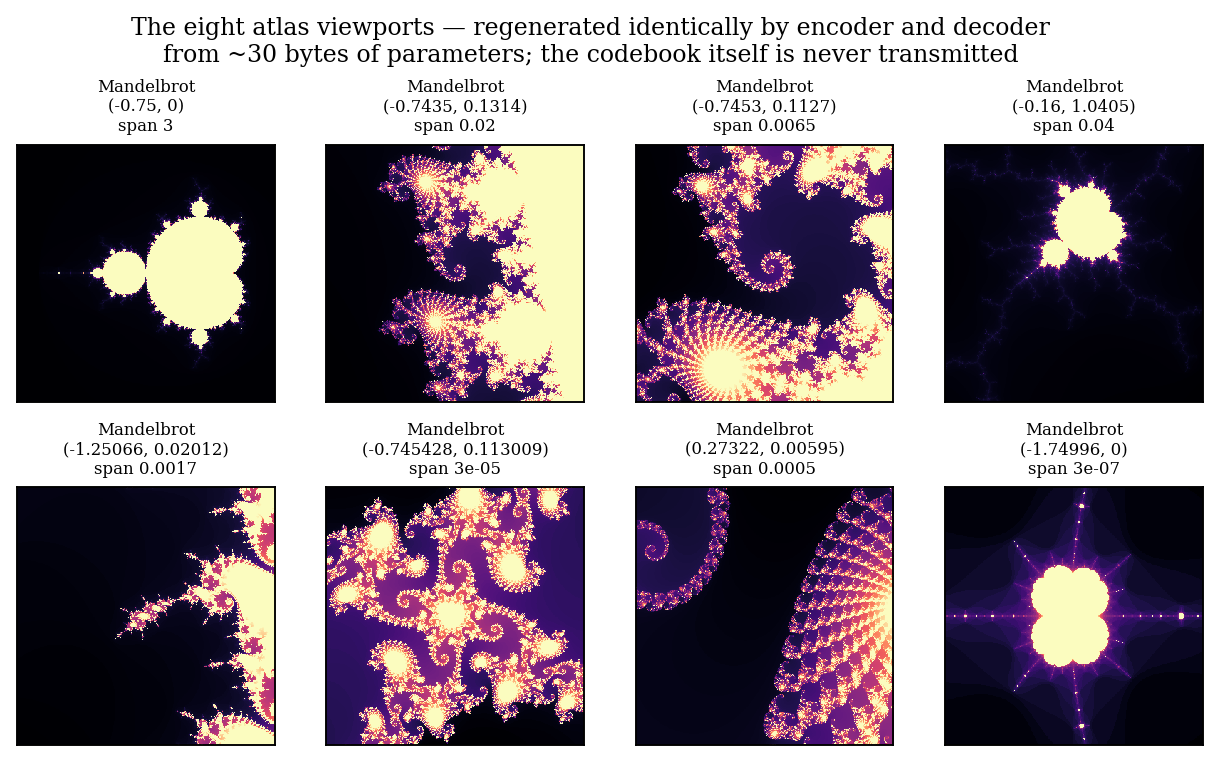
\includegraphics[width=\textwidth]{fig_atlas.png}
\caption{The eight atlas viewports. Each is fully determined by 3--5 numbers;
the whole codebook regenerates from ${\sim}30$ bytes of parameters and is never
transmitted. Boundary regions are chosen because escape-time values there are
\emph{textured}: ramps, plateaus, oscillations and rough noise, at every scale.}
\label{fig:atlas}
\end{figure}

\begin{figure}[t]
\centering
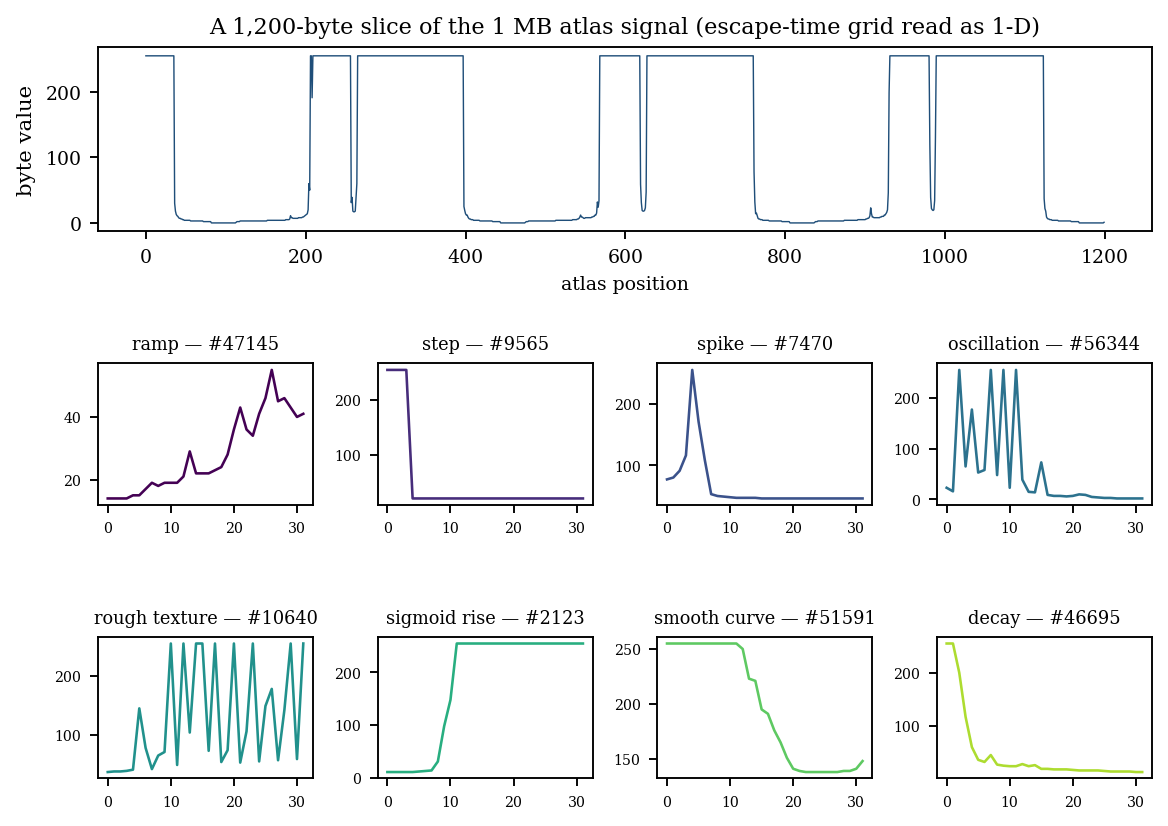
\includegraphics[width=0.95\textwidth]{fig_bank.png}
\caption{Top: a structured slice of the atlas read as a 1-D byte signal.
Bottom: eight of the 65{,}535 candidate windows, one exemplar per local-shape
family --- ramp, step, spike, oscillation, rough texture, sigmoid rise, smooth
curve, decay. The bank behaves as a universal library of local shapes.}
\label{fig:bank}
\end{figure}

From the atlas the codec extracts \textbf{65{,}535 candidate windows} (so an
address fits in two bytes). Crucially, the bank is \emph{multi-scale}: windows
are read at $1\times$, $2\times$, and $4\times$ dilation
(Figure~\ref{fig:multiscale}). Because the fractal is self-similar, dilated
reads are not blurry copies but \emph{genuinely new shapes} --- the defining
property of the fractal doing real compression work. This single change
extended the codec's winning range from 256\,B to 1\,KB.

\begin{figure}[t]
\centering
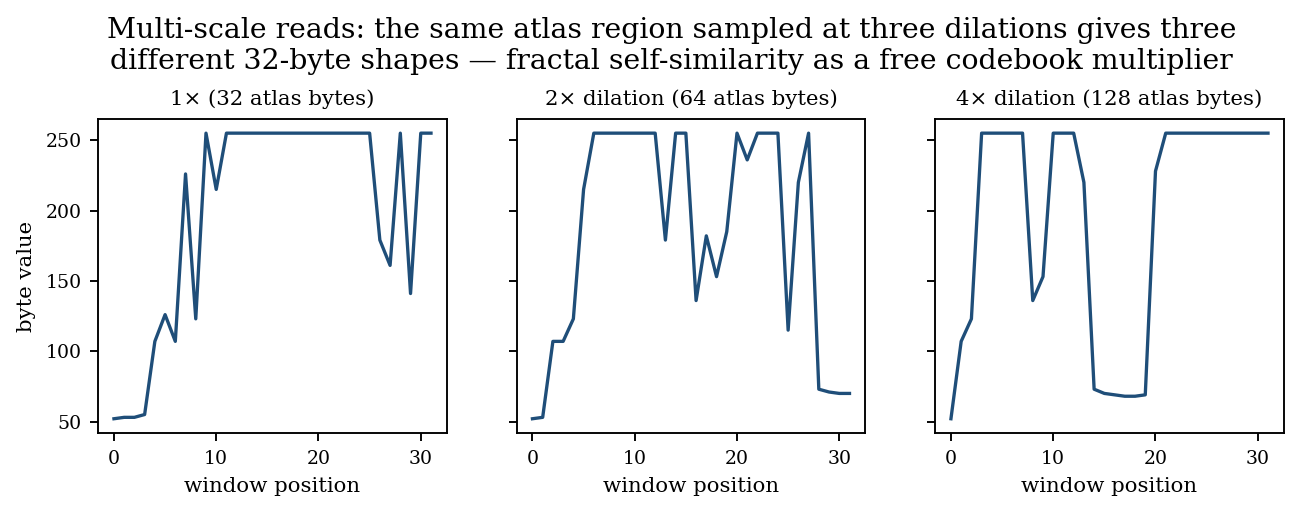
\includegraphics[width=\textwidth]{fig_multiscale.png}
\caption{Multi-scale reads. The same atlas offset sampled at three dilations
yields three distinct 32-byte shapes: self-similarity acts as a free codebook
multiplier.}
\label{fig:multiscale}
\end{figure}

\section{The codec: address + fit + correction}
\label{sec:codec}

Figure~\ref{fig:pipeline} shows the pipeline. The input is split into 32-byte
blocks; for each block the encoder:

\begin{enumerate}
\item \textbf{Searches} the bank for the window with the highest absolute
normalized correlation (a vectorized $65{,}535$-way match;
Figure~\ref{fig:match}, left).
\item \textbf{Fits} the window to the block with a two-parameter affine map
$\hat{x} = s\cdot w + o$: a quantized scale $s$ (1 byte, including
\emph{negative} scales --- an upward fractal ramp can model a downward audio
slope) and an offset $o$ (sent as a delta between consecutive blocks, since
block means drift smoothly; Figure~\ref{fig:match}, middle). A per-block mode
bit lets a plain linear ramp replace the fractal patch wherever a straight
line predicts better --- smooth blocks are cheaper that way.
\item \textbf{Corrects}: the residual between prediction and truth is wrapped
to $[-128,127]$, zigzag-mapped so small magnitudes become small unsigned
integers, and entropy-coded (Figure~\ref{fig:match}, right).
\end{enumerate}

\begin{figure}[t]
\centering
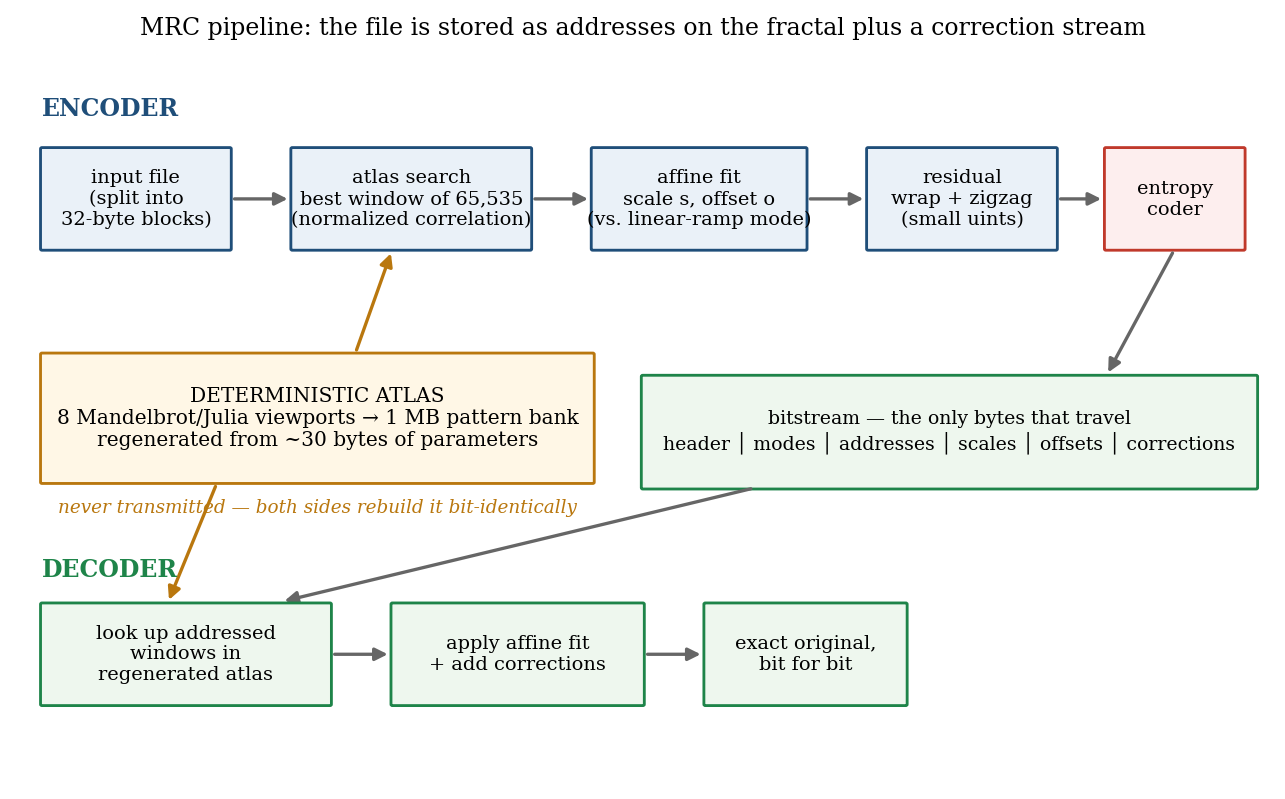
\includegraphics[width=\textwidth]{fig_pipeline.png}
\caption{The MRC pipeline. Only the green bitstream travels; the orange atlas
is rebuilt independently on each side.}
\label{fig:pipeline}
\end{figure}

\begin{figure}[t]
\centering
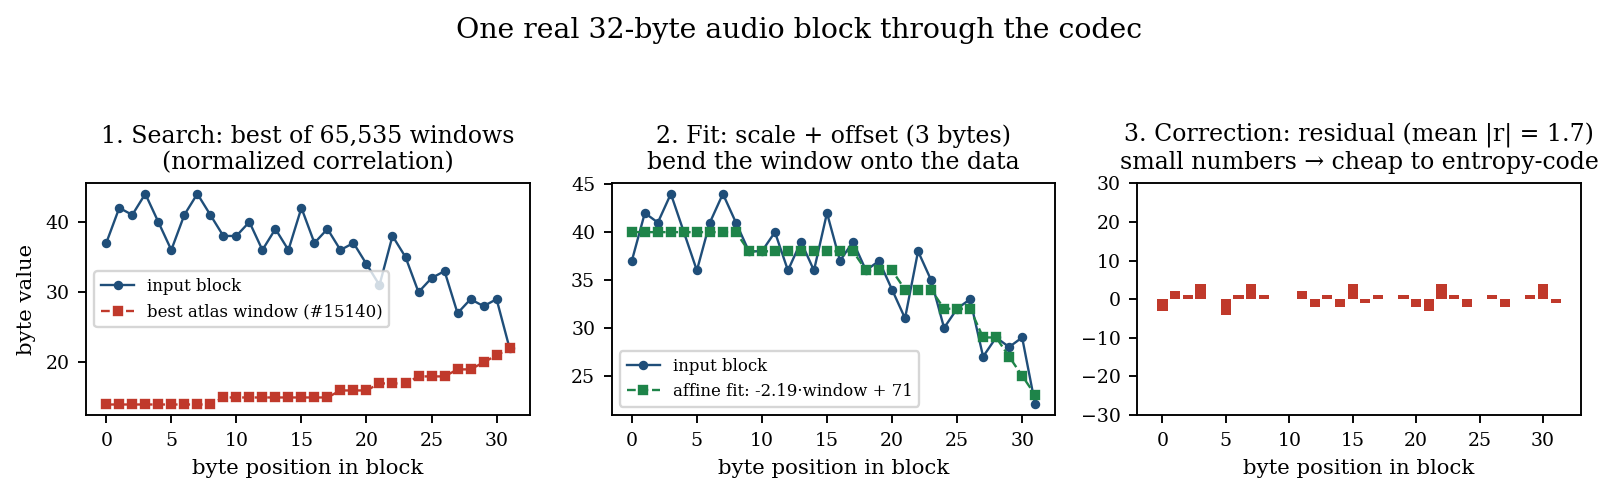
\includegraphics[width=\textwidth]{fig_match.png}
\caption{A real 32-byte block of PCM audio through the codec. The best atlas
window (left) is fit with scale $-3.25$ and offset $350$ (middle) --- note the
flip: a rising fractal ramp models a falling audio slope. The remaining
residual (right) has mean magnitude $1.6$, costing only a few bits per byte
after entropy coding.}
\label{fig:match}
\end{figure}

The decoder reverses the process with no search: it regenerates the atlas,
looks up each address, applies the stored fit, and adds the corrections. The
output is the original file, bit for bit --- verified by roundtrip on every
encode in every benchmark reported here.

\subsection{Entropy coding and container selection}

Addresses, scales, modes and offset deltas (``side information'') compress well
under LZMA in raw framing --- the standard \texttt{.xz} container alone costs
${\sim}55$ bytes, an enormous tax at these sizes, so MRC strips it. The
correction stream gets a purpose-built \textbf{adaptive range coder} whose
byte model starts from a geometric prior (half-life 3) matched to zigzag
residual statistics --- worth $-4\,\%$ over a flat prior. An LZMA-style
adaptive bit-tree coder was implemented and \emph{lost} to this model on small
payloads; we keep the negative result on record.

The encoder then performs a \textbf{container choice}
(Figure~\ref{fig:format}) over every format family: the engine stream (raw
LZMA or range-coded, plain or byte-plane-deinterleaved), the delta transforms
(byte delta, and int16 sample delta in either entropy coder), whole-stream
LZMA and plane-delta, and stored (for incompressible input) --- ten formats
in v2.4, grown from the original four. One format byte makes the choice
self-describing, and guarantees the codec never loses meaningfully to its
own baselines.

\begin{figure}[t]
\centering
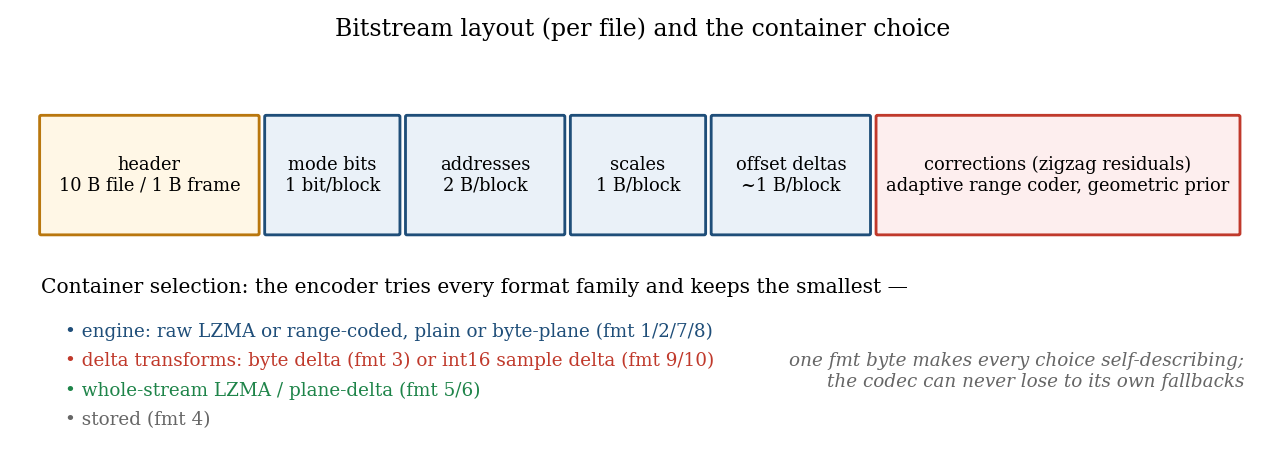
\includegraphics[width=\textwidth]{fig_format.png}
\caption{Bitstream layout and the container selection across format families.}
\label{fig:format}
\end{figure}

\subsection{Frame mode}

For transport-framed payloads --- BLE, radio, UDP, where the transport already
knows the length --- a dedicated mode shrinks the header to \textbf{one byte}
and packs mode bits, raw addresses and scales, then runs a single adaptive-AC
pass over offset escapes plus corrections. This is the regime where every
byte of framing matters most. For int16 sensor streams a second frame family
(sample-delta $\to$ zigzag $\to$ byte-plane split $\to$ range coder) handles
data whose structure lives between \emph{samples} rather than bytes; v2.4
unifies both families under the same one-byte header
(Section~\ref{sec:v24}).

\subsection{Variable-block segmentation}
\label{sec:varblock}

A fixed 32-byte block is the wrong unit almost everywhere: where one atlas
shape fits a long stretch of signal, fixed blocks pay address-and-fit
side-information 32 bytes at a time; where the signal is busy, even 32 bytes
is too coarse. v2.3 therefore lets the encoder choose each block's size from a
power-of-two ladder (32--512 bytes). A bottom-up dynamic program over each
span compares the estimated coded cost of one large block against the best
split into its two halves, recursively; the cost model is the per-block
side-information plus an Elias-gamma-style estimate of the residual bits.
Because the expensive per-level predictions are computed once, the encoder
runs the (cheap) DP at four side-cost settings and keeps the smallest result.
The chosen layout is signalled as one ${\sim}2$-bit symbol per block which
LZMA compresses further; the decoder reads this stream and re-derives every
cut exactly --- \textbf{no per-chunk headers, no length fields}
(Figure~\ref{fig:varblock}).

\begin{figure}[t]
\centering
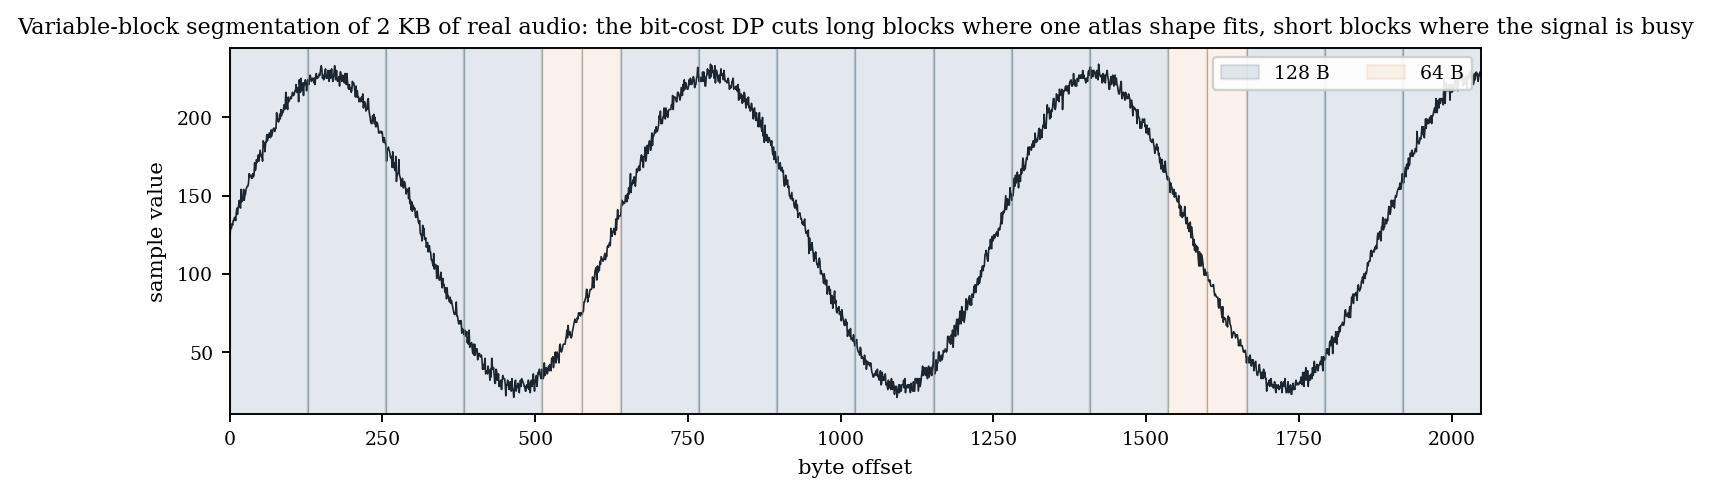
\includegraphics[width=\textwidth]{fig_varblock.png}
\caption{The dynamic program segmenting 2\,KB of real audio. Long blocks
cover stretches one affine-fitted atlas shape can predict; short blocks
appear where the signal misbehaves. The layout costs ${\sim}2$ bits per block
to transmit.}
\label{fig:varblock}
\end{figure}

The motivation came from a measured negative result (Section~\ref{sec:neg}):
cutting a large file into \emph{independent} MRC chunks loses 14--39\,\%,
because each chunk pays its own entropy-coder warm-up and is blind to
long-range structure. Variable blocks keep the single shared entropy pass and
the single offset-delta chain --- one seamless encode --- while still letting
the \emph{cut sizes} adapt to the data. The same idea, moved inside the
container, is what extends the codec's range (Section~\ref{sec:large}).
Additionally, v2.3 lifts the range coder's size cap: the geometric-prior
adaptive coder beats raw-LZMA framing on correction streams at every size we
measured (e.g.\ 29{,}746 vs.\ 30{,}761 bytes on a 64\,KB audio correction
stream).

\section{Results}
\label{sec:results}

All numbers compare MRC against the \emph{best per slice} of gzip-9, LZMA-9e
(\texttt{PRESET\_EXTREME}), and delta+LZMA --- i.e.\ against an oracle that
always picks the strongest classical baseline. The benchmark covers 7 sources
$\times$ 4 sizes $\times$ 5 random offsets (140 slices).

\subsection{The small-payload regime}

MRC wins \textbf{132 of 140} slices (Figure~\ref{fig:bench}, left); all eight
losses are sub-1\,KB slices of the smooth coastline source. At 256 bytes the
margins on textured data average 19--36\,\% (best single slice: audio at
$+40.1\,\%$); at 512\,B--1\,KB, 10--27\,\% across every textured source. By
4\,KB the margin is 2--7\,\% --- and on audio it is now the fractal engine
itself winning there, not the fallback container, a direct effect of
variable-block segmentation (Section~\ref{sec:varblock}).

\begin{figure}[t]
\centering
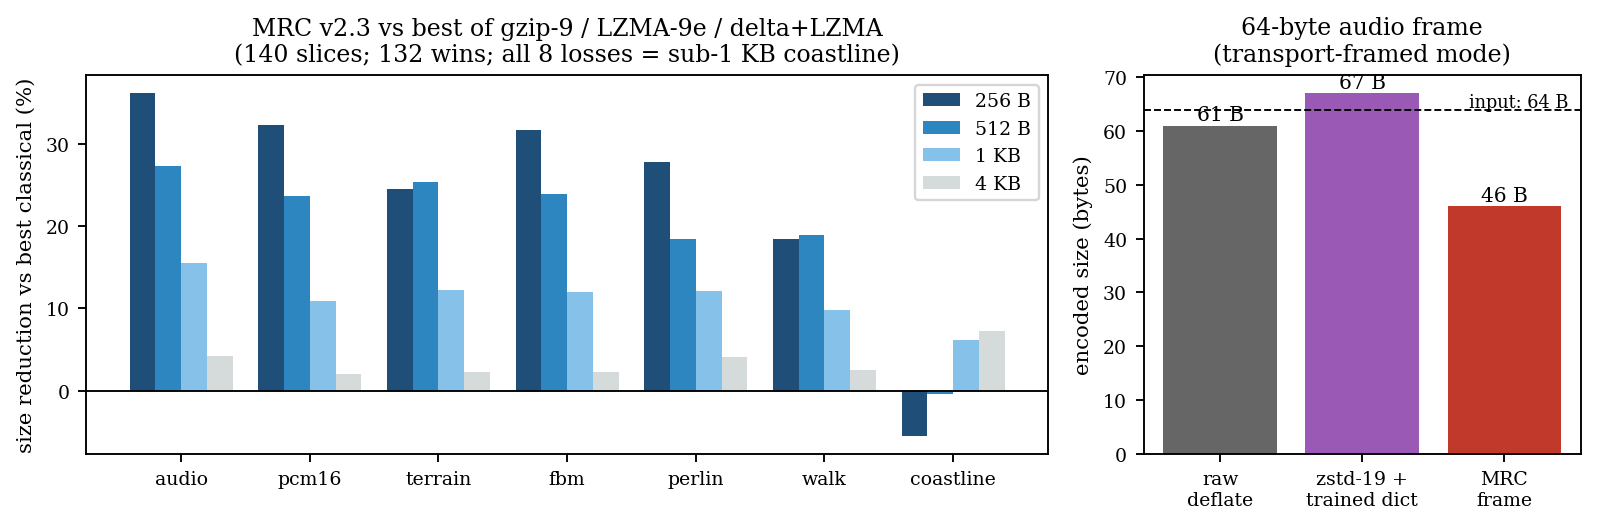
\includegraphics[width=\textwidth]{fig_bench.png}
\caption{Left: savings vs.\ the best classical baseline per source and size.
Right: the frame-mode knockout on 64-byte audio frames --- MRC's 46 bytes
against deflate's 61 and dictionary-equipped zstd-19's 67.}
\label{fig:bench}
\end{figure}

\subsection{Against trained dictionaries}

The strongest classical answer to the small-file problem is zstd with a
\emph{trained dictionary} --- which plays exactly MRC's game, except the
dictionary (21--112\,KB in our tests) must be provisioned on both sides. Even
granting zstd magic-less, checksum-less framing, \textbf{MRC frame mode wins
96 of 96 frames by 25--40\,\%}. The reason is structural: trained dictionaries
exploit \emph{exact repeats} of training data, and textured signals contain
none; MRC's affine approximate matching does not care --- it needs shapes, not
repeats.

\subsection{Large files: the variable-block extension}
\label{sec:large}

Fixed-block MRC had no edge above ${\sim}4$\,KB: classical compressors get
room to build their own dictionary, and the v2.2 codec silently became its
delta+LZMA fallback (a 0.0\,\% tie at 256\,KB). Variable-block segmentation
changes this on real data. A decomposition of the v2.2 stream at 64\,KB shows
why: the fractal \emph{corrections} alone were already smaller than
delta+LZMA's whole output --- the entire deficit was per-block
side-information, and larger blocks attack exactly that term. With the
32--512-byte ladder, the fractal stream beats the best classical baseline on
audio at every size tested:

\begin{center}
\small
\begin{tabular}{lrrr}
\toprule
 & best classical & MRC v2.3 & margin \\
\midrule
16\,KB  & 8{,}748   & \textbf{8{,}564}   & $+2.1\,\%$ \\
64\,KB  & 34{,}392  & \textbf{33{,}767}  & $+1.8\,\%$ \\
256\,KB & 137{,}212 & \textbf{133{,}774} & $+2.5\,\%$ \\
\bottomrule
\end{tabular}
\end{center}

We scope this honestly: the large-file fractal win holds on \emph{real audio}.
The synthetic sources (terrain, fBm, Perlin, random walk) still drop to the
fallback container at 16\,KB and above, winning only 0.0--2.2\,\% on container
thrift. The claim is therefore not ``MRC beats LZMA on large files'' but
``variable-block MRC extends the fractal engine's winning regime through
256\,KB on textured real-world signals.''

\subsection{Where it does not win}
\label{sec:neg}

Three negative results, measured rather than argued
(Figure~\ref{fig:regime}):

\begin{description}
\item[Independent chunking does not transfer the edge.] Cutting a large file
into 256\,B--1\,KB pieces and concatenating MRC frames loses \textbf{14--39\,\%}
versus whole-file encoding (audio and PCM corpora). Each chunk pays its own
warm-up, and chunks are blind to the long-range redundancy LZMA sees whole.
This negative result is what motivated Section~\ref{sec:varblock}: adapt the
cut sizes \emph{inside} one seamless encode instead of cutting the encode
itself.
\item[Smooth data.] All eight benchmark losses are sub-1\,KB coastline
slices ($-6$ to $-8\,\%$ at 256\,B): a smooth curve needs no texture
codebook, and the affine-fit machinery is pure overhead there. The fallback
container caps the damage and wins the source back by 1\,KB.
\item[2-D tiles.] A tile-reordered 2-D mode with true 2-D atlas patches
roundtrips correctly but loses 8--9\,\% to the 1-D path on smooth heightmaps:
tile reordering destroys more long-range structure than 2-D patches add.
Untested on photographs.
\end{description}

\begin{figure}[t]
\centering
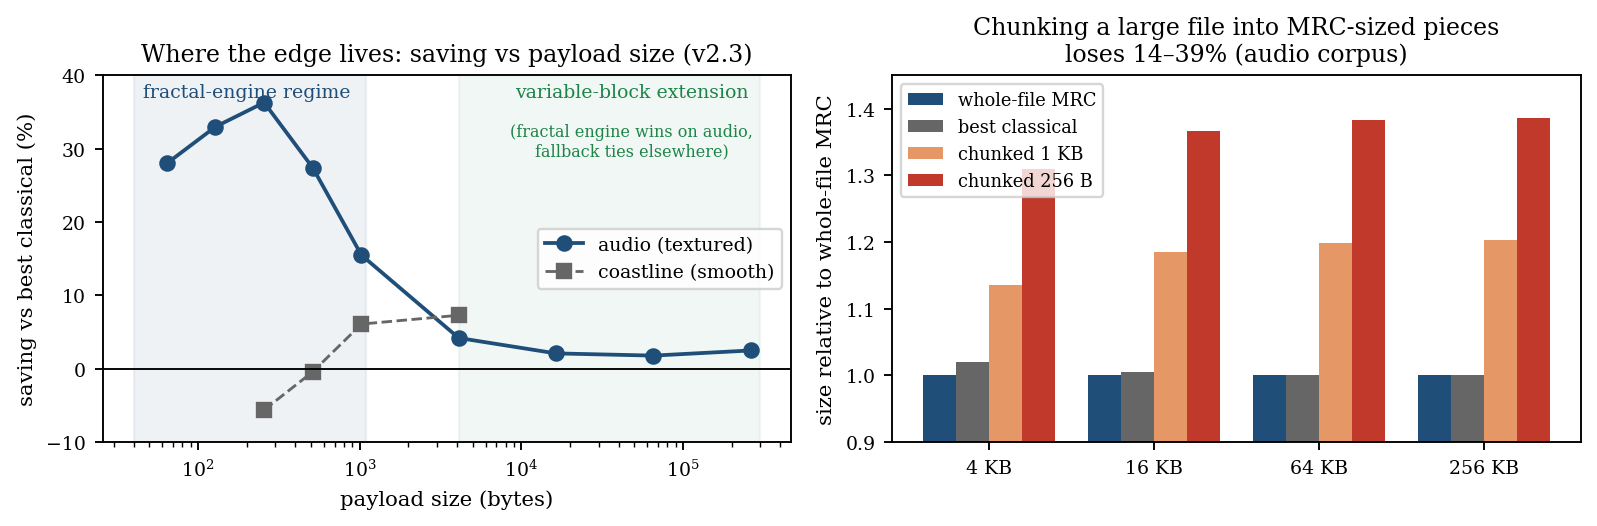
\includegraphics[width=\textwidth]{fig_regime.png}
\caption{Left: the niche, mapped --- savings peak in the 64\,B--1\,KB window on
textured data; with variable blocks the audio edge no longer decays to zero
but holds at $+1.8$--$2.5\,\%$ through 256\,KB. Smooth data (coastline) is
ambivalent. Right: chunking large files into \emph{independent} MRC pieces is
strictly worse than whole-file encoding at every size and every chunk size
tested --- the negative result that motivated variable-block segmentation.}
\label{fig:regime}
\end{figure}

\section{Real-world telemetry}
\label{sec:real}
\label{sec:realdata}

The benchmark above is dominated by audio and synthetic textures. To test the
intended deployment --- constrained-transport sensor telemetry --- we added two
real corpora: \textbf{seismometer ground vibration} (IRIS network, 40\,Hz and
100\,Hz channels, int16 counts) and \textbf{machine-bearing acceleration}
(CWRU corpus, healthy and faulted, full bandwidth).

Real data immediately earned its keep: a 256-byte seismometer slice starting at
an \emph{odd} byte offset misaligns the int16 view, neighbouring ``samples''
jump by more than $\pm 32767$, and the sample-delta transform's zigzag output
silently overflowed its 16-bit container --- a lossless codec that wasn't. The
synthetic suite never produced the case. The fix wraps each delta into int16
range before zigzag (congruent modulo $2^{16}$, so the decoder's existing
cumulative sum recovers the exact samples); all results below post-date the fix
and, as everywhere in this paper, every encode is roundtrip-verified.

On seismometer data MRC saves \textbf{17--34\,\%} on 256\,B--1\,KB slices
against the best classical baseline (which here includes a hand-rolled
int16-aware sample-delta+LZMA --- the strongest thing a competent firmware
engineer would write), and \textbf{${\sim}47\,\%$ on 64-byte transport frames}:
33.6 bytes mean where raw deflate manages 59.5 and the int16-aware baseline
44.6. Bearing acceleration at full bandwidth is the honest negative: near
incompressible for every method (0--7\,\%), and MRC correctly degrades to its
stored fallback rather than pretending. Notably, on this telemetry the winning
formats are mostly the \emph{atlas-free} sample-delta paths --- a fact that
motivates the next section's question.

\section{Is the Mandelbrot set special?}
\label{sec:zoo}

The architecture requires only that the codebook be \emph{deterministically
regenerable from a tiny seed}. Nothing requires it to be the Mandelbrot set.
We therefore ran \textbf{nineteen} same-size (1\,MB) codebooks through the
otherwise identical pipeline --- same multi-scale windowing, same affine fit,
same containers --- on the same 72 slices and 96 frames
(Figure~\ref{fig:zoo}): the Mandelbrot atlas; three seeded-PRNG baselines
(white noise, Brownian walk, spectral $1/f$ noise); and fifteen alternative
constructions (Newton basins, four Julia sets, Sierpinski as Pascal's triangle
mod 256, flower-of-life circle lattice, Cantor staircase, Barnsley fern,
Burning Ship, Koch, dragon and L\'evy curves, Takagi, Weierstrass, Lorenz
attractor, logistic-map orbit, and a Hilbert-scanned Mandelbrot).

\begin{figure}[t]
\centering
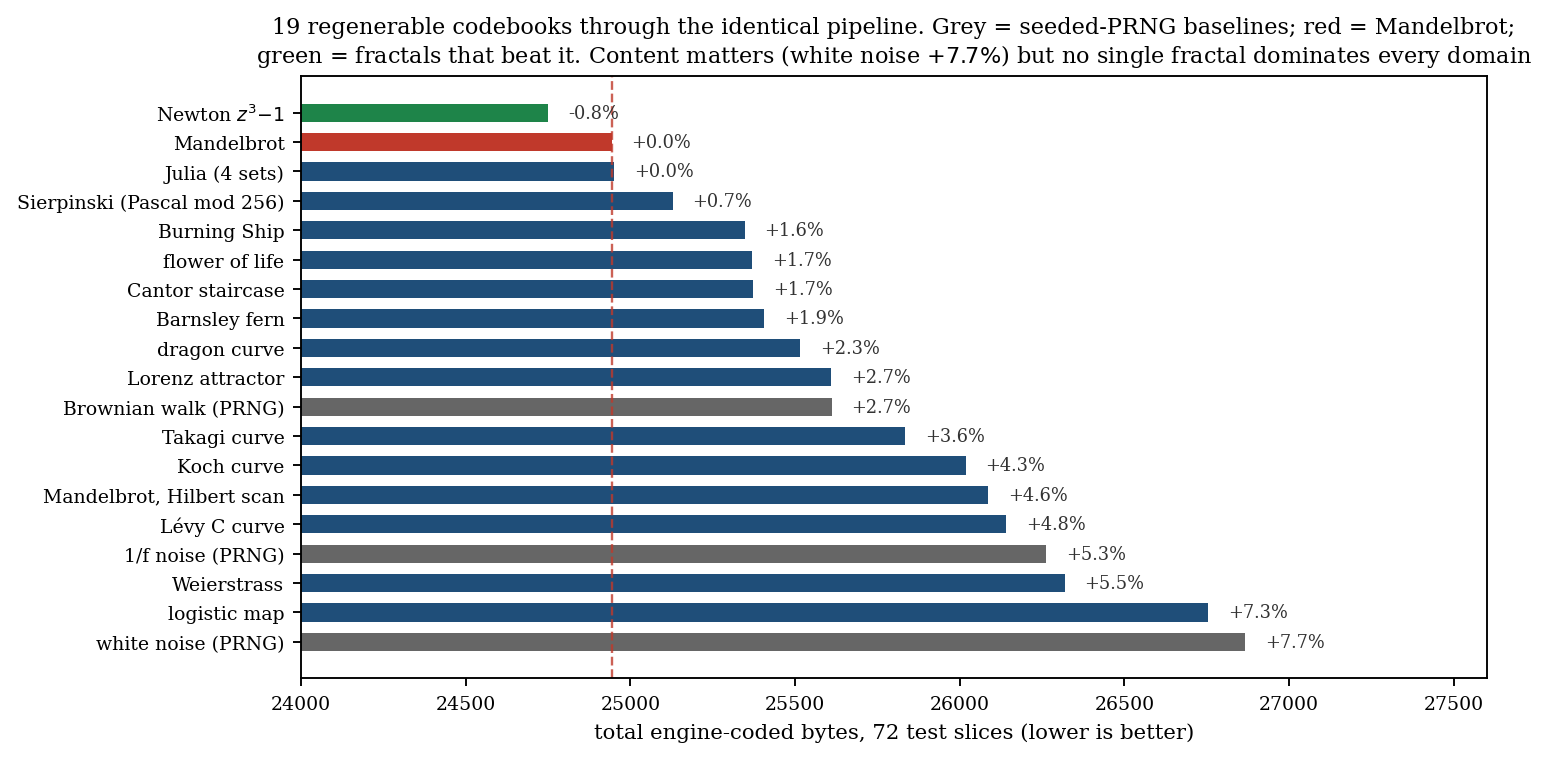
\includegraphics[width=\textwidth]{fig_zoo.png}
\caption{The codebook-content study. Every bar is the same engine with only
the regenerated codebook swapped.}
\label{fig:zoo}
\end{figure}

Five findings, each measured:

\begin{description}
\item[Content matters.] White noise costs $+7.7\,\%$ over the Mandelbrot atlas
(and on seismic slices $+12\,\%$); the engine barely selects it on audio (3--9\,\%
of blocks vs.\ 76--92\,\% for the fractal). The codebook is doing real work.
\item[But cheap structure closes most of the gap.] A one-line Brownian walk
comes within $2.7\,\%$ overall. Claims that the Mandelbrot set is
\emph{uniquely} suited would be overclaiming; we make no such claim.
\item[No fractal wins everywhere --- they specialize.] Newton basins of
$z^3{-}1$ beat Mandelbrot overall ($-0.8\,\%$) and on seismic slices
($-2.8\,\%$); the flower-of-life lattice wins \emph{every} audio and PCM row
($-2.8$ to $-4.4\,\%$) yet loses every seismic row; Sierpinski wins frame mode
outright ($-6.6\,\%$) with seismic residuals \emph{half} of Mandelbrot's.
Smooth-arc codebooks fit waveforms; arithmetic-textured codebooks fit
byte-plane structure; basin-boundary texture fits broadband vibration.
\item[Blending fails; selection works.] A composite atlas greedily assembled
from chunks of all nineteen (driven by the residual-energy proxy) beat the
incumbent on its training data and lost by $3.7\,\%$ held-out --- the second
proxy failure (cf.\ Section~\ref{sec:atlas}). Per-item \emph{selection} among
whole codebooks, scored by actual encoded bytes, is what works
(Section~\ref{sec:v24}).
\item[Reading order is load-bearing.] The same Mandelbrot content scanned along
a Hilbert curve --- ``better'' 2-D locality in 1-D --- loses $4.6\,\%$ to plain
row order. Negative, on record.
\end{description}

\section{v2.4: a registry of regenerable codebooks}
\label{sec:v24}

v2.4 turns the zoo's complementarity into bytes. The format gains a
\textbf{codebook ID}: one extra header byte in the container (MRC4; MRC3
streams remain decodable), and \emph{zero} extra bytes in frame mode, where the
ID rides in spare format-code space of the existing one-byte header. The
registry holds four specialists --- Mandelbrot (ID 0, legacy), Newton,
flower-of-life, Sierpinski --- each regenerated on demand exactly like the
original atlas; the decoder regenerates whichever codebook the ID names. The
encoder simply tries the engine under each codebook plus the atlas-free
transforms and keeps the global minimum: ${\sim}4\times$ the encode compute,
zero decode cost beyond regenerating one more codebook. The same release
unifies the two frame families (atlas-engine and sample-delta) under one
header, so every frame gets the better of both.

Held-out results (second halves of all four real sources, fresh offsets,
end-to-end encoded bytes; Figure~\ref{fig:v24}): slices $-2.1\,\%$ (audio
$-3.2\,\%$, PCM $-3.8\,\%$; seismic flat because the atlas-free transforms
already win there), frames $-6.2\,\%$ (seismic $-9$ to $-10\,\%$). The
optimistic bound measured on the corpus the roster was selected on is
$-2.2\,\%$/$-7.1\,\%$ --- within noise of the held-out numbers, i.e.\ the gain
generalizes. The selection statistics confirm genuine division of labour:
on held-out frames Sierpinski wins 45 of 96, Mandelbrot 21, Newton 17; on
slices the flower-of-life lattice takes essentially every slice where the
engine beats the transforms. A 400-case randomized roundtrip fuzz (odd
offsets, all sizes, both frame families) passes with zero failures.

\begin{figure}[t]
\centering
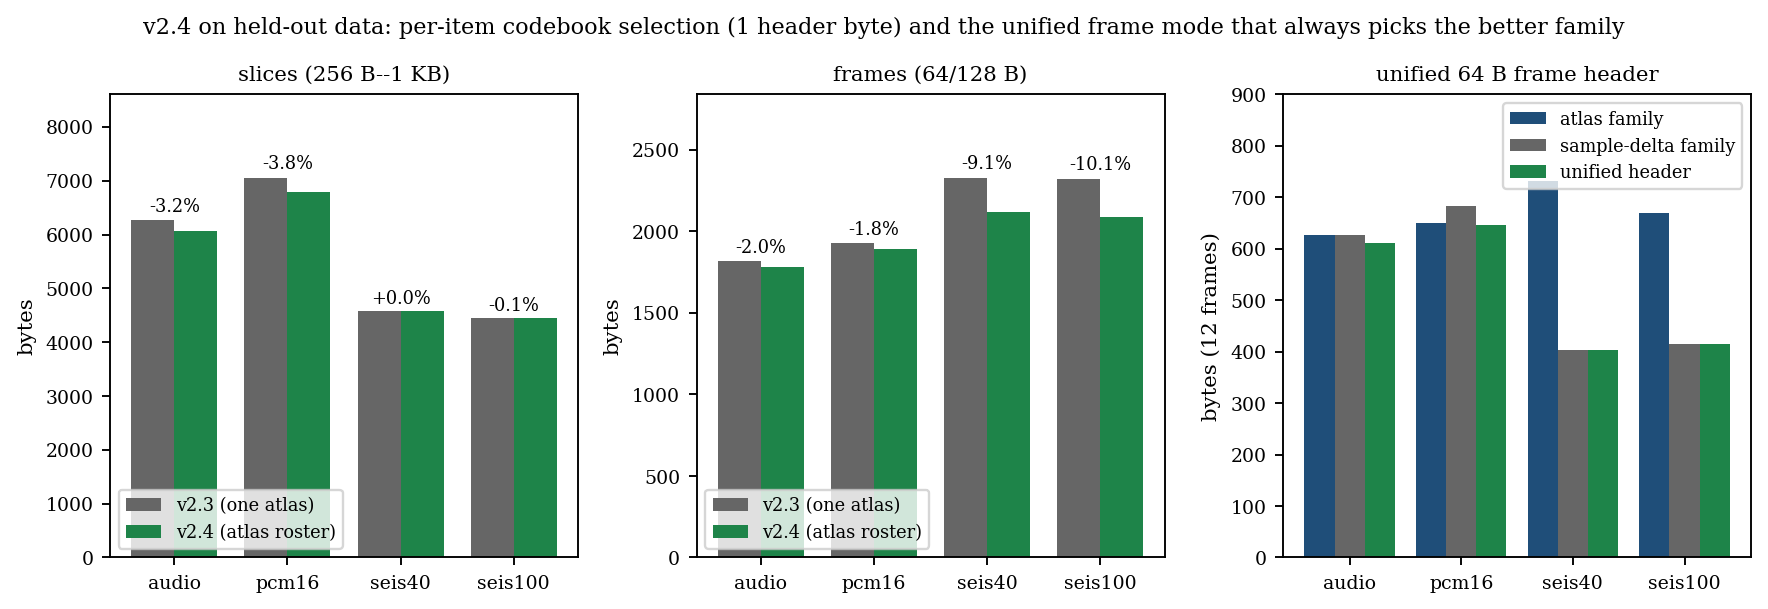
\includegraphics[width=\textwidth]{fig_v24.png}
\caption{v2.4 held-out results: codebook selection per item, and the unified
frame header picking the better frame family per frame.}
\label{fig:v24}
\end{figure}


\section{Growing the registry: hunted and designed codebooks}
\label{sec:registry-growth}

The registry's open-endedness was exercised twice in the days after v2.4
shipped, in two different modes: \emph{hunting} (testing fixed generator
families) and \emph{designing} (searching a family's parameter space per use
case). Both rounds kept the discipline of Section~\ref{sec:zoo}: candidates
are scored by real encoded bytes, and nothing ships without beating the
incumbent on held-out data it was never selected on. Figure~\ref{fig:registry}
shows the resulting eight-codebook catalog side by side.

\begin{figure}[t]
\centering
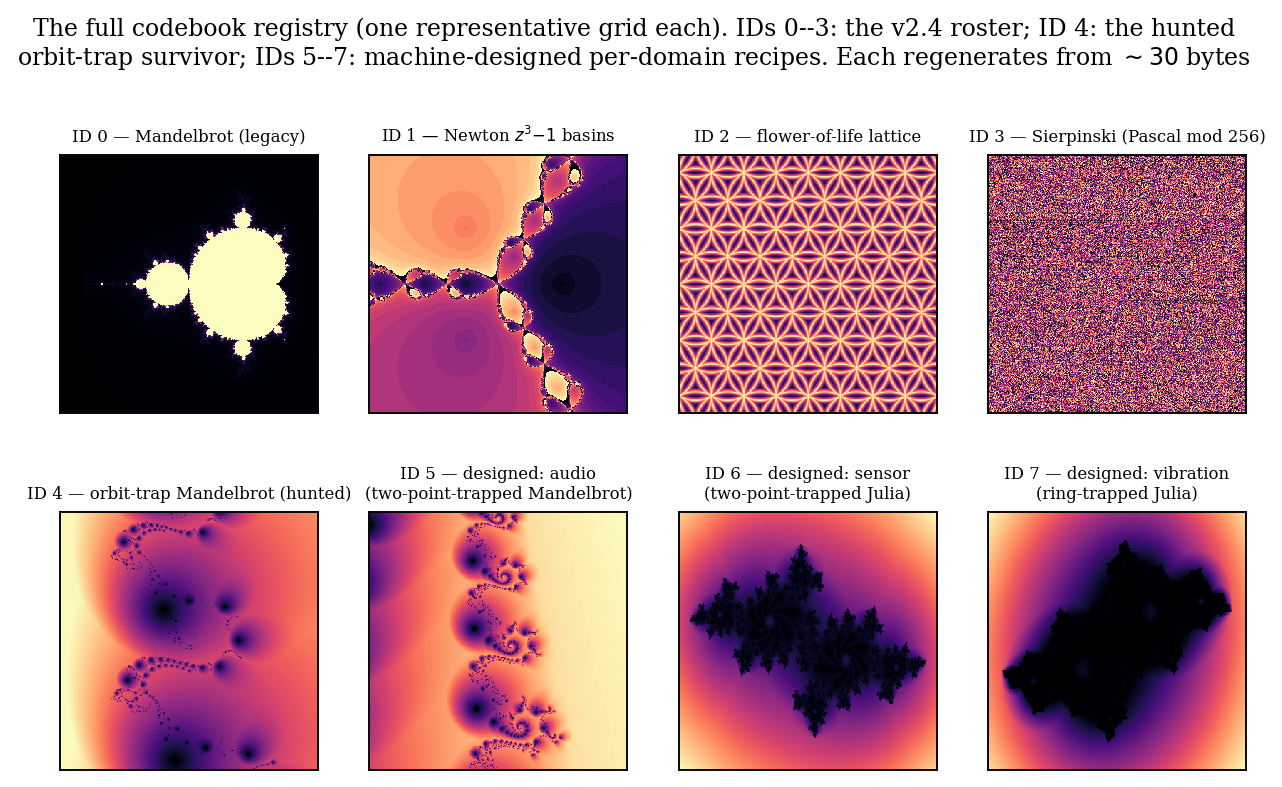
\includegraphics[width=\textwidth]{fig_registry.png}
\caption{The full codebook registry, one representative $362\times362$ grid
each. IDs 0--3 are the v2.4 roster (Section~\ref{sec:v24}); ID 4 is the hunted
orbit-trap survivor; IDs 5--7 are the machine-designed per-domain recipes.
Every codebook regenerates deterministically from ${\sim}30$ bytes of
parameters --- nothing here is ever transmitted.}
\label{fig:registry}
\end{figure}

\subsection{Hunting: twelve new families, one survivor}

A third zoo round tested twelve families absent from the original study:
eight chaotic-attractor time series (H\'enon, Clifford, Ikeda, Chirikov,
Thomas, R\"ossler, Halvorsen, forced Duffing), three new escape-time grids
(burning ship, tricorn, multibrot $z^3$), and two continuous renders of the
Mandelbrot recipe (smooth fractional iteration, orbit-trap distance). The
attractor hypothesis --- that smooth oscillatory texture fits waveforms
better than escape terraces --- failed decisively: every attractor lost by
$+4$ to $+7\,\%$. The codec does not want codebook texture that
\emph{resembles} the signal; the affine fit supplies the waveform shaping,
and what the codebook must supply is multi-scale detail, which escape-time
terraces have and smooth orbits lack. Multibrot $z^3$ led the probe corpus
and surrendered its lead on held-out data --- the same selection-mirage the
two-phase protocol caught twice before. The sole survivor was the
\textbf{orbit-trap render} ($-0.9\,\%$ engine bytes held-out, but $+6\,\%$ on
frames, where Sierpinski remains best), shipped as registry ID 4. A fourth
round probed twelve orbit-trap variants (trap shapes, Julia/burning-ship/%
multibrot bases, mean aggregation); the best edged the incumbent by amounts
within noise while losing on frames, so the registry was left unchanged ---
a vein struck, mined, and exhausted in two rounds.

One engineering honesty note: in frame mode the encoder \emph{does} try every
roster codebook per frame (that is how v2.4's gains arise), so roster size is
a linear encode-time cost --- measured $45\!\to\!91$\,ms/frame in the
reference implementation when a fifth codebook joins the roster, for zero
gain on seismic data. The registry therefore distinguishes the \emph{catalog}
(all defined IDs; free) from the \emph{roster} a deployment actually
searches (chosen per data class; costed). IDs 4--7 are catalog members that
deployments opt into.

\subsection{Designing: a codebook per use case}

The fifth round inverted the question: instead of asking which fixed
generator suits a domain, \emph{search the generator's parameter space
against that domain}. For each of four domains --- audio, sensor PCM,
seismic, vibration --- 25 candidate recipes were drawn from five
parameterized families (orbit-trapped Mandelbrot with free trap shape, trap
point and viewports; orbit-trapped Julia sets with $c$ sampled near the
cardioid boundary; smooth-escape Mandelbrot; Pascal's triangle mod $m$;
circle-lattice fields with free radius, decay and spans). Fitness was real
encoded bytes on a probe corpus; the top two recipes per domain were then
re-scored on held-out data against the best champion for that domain.

Designed recipes won three of four domains: audio $-0.7\,\%$ (a
two-point-trapped Mandelbrot), sensor $-0.6\,\%$ (two-point-trapped Julia
sets), vibration $-0.6\,\%$ (ring-trapped Julia sets); seismic stayed with
Sierpinski ($+0.5\,\%$ for the best designed candidate). One sensor finalist
that led the probe corpus failed held-out replication and was discarded.
The three winners ship as registry IDs 5--7. Two properties matter. First,
each remains a ${\sim}30$-parameter deterministic recipe --- the search
selects parameters, it does not learn data, so the zero-shipped-dictionary
property of Section~\ref{sec:atlas} survives machine design. Second, the
vibration result is qualitatively new: bearing data that every codec in
Section~\ref{sec:real} found near-incompressible still yielded a measurable,
held-out-verified gain to a recipe designed for it. The margins are small
(sub-$1\,\%$, like every codebook refinement since v2.4) and 25 random draws
per domain is a deliberately small first search; the result establishes the
mechanism --- per-domain codebook design under full-encoder scoring and
held-out validation --- rather than its ceiling.

\section{Why it works}
\label{sec:why}

The result is best understood through the dictionary-bootstrap lens of
Section~1. Classical coders amortize a learned model over the file; below
${\sim}1$\,KB there is nothing to amortize against. MRC moves the model
\emph{out of the channel entirely}: the fractal is an infinitely detailed,
deterministically shared prior, and the only per-file cost is pointing into
it. Four properties make the Mandelbrot family a good universal prior for
textured 1-D signals:

\begin{enumerate}
\item \textbf{Boundary texture.} Escape-time fields near the boundary contain
ramps, plateaus, oscillations and broadband roughness --- the local vocabulary
of real sensor and audio data.
\item \textbf{Self-similarity.} Dilated reads of the same field are new,
valid shapes, multiplying the codebook at zero parameter cost
(Figure~\ref{fig:multiscale}).
\item \textbf{Affine closure.} With a scale-and-offset fit (negative scales
included), one stored shape models a whole equivalence class of blocks; the
mode bit covers the degenerate class (straight lines) even more cheaply.
\item \textbf{Adaptive granularity.} Self-similarity also means a good match
exists at \emph{many} block lengths; the segmentation DP exploits this,
spending side-information only where the signal demands it. This is what
carries the engine past its former 4\,KB ceiling.
\end{enumerate}

What the fractal does \emph{not} provide is your file's specific long-range
structure --- exact repeats, periodicities at lag 512, cross-row correlations.
That is exactly the information classical dictionary coders harvest, which is
why the regimes partition so cleanly and why the honest product is a codec
with classical fallbacks built in.

Section~\ref{sec:zoo} sharpens the claim. The four properties above are not
exclusive to the Mandelbrot set --- Newton basins and even a circle lattice
exhibit them, each with a different texture bias --- and that is the point:
\textbf{the invention is the architecture}, a codebook that is computed rather
than shipped, addressed approximately, and corrected exactly. \emph{Which}
mathematics generates the codebook is a tunable degree of freedom, and v2.4
exposes it in one header byte. This also positions MRC honestly against prior
art: algebraic codebooks in speech coding~\cite{acelp}, an expired patent on
RNG-regenerated dictionaries~\cite{aronov}, and relative-entropy coding's
shared-seed codebooks~\cite{rec} each contain one ingredient; the measured
combination --- fixed mathematical generators, multi-scale approximate match,
exact correction, per-item generator selection --- is, to our knowledge, new.

\section{Limitations and outlook}

MRC v2.4 is a Python/NumPy research codec: encode of a 256\,KB file takes
${\sim}$half a minute per codebook (the multi-level 65{,}535-way correlation
dominates); decode is already search-free and fast. A first C port of the
frame encoder --- bitstream-identical to the reference, 240/240 byte-exact
parity --- measures 2.3\,ms per 64-byte frame for a single codebook and
9.6\,ms for the four-codebook roster on one low-power x86 core (vs.\ 93\,ms
in Python), with the sample-delta family at ${\sim}1\,\mu$s per frame:
real-time for 8\,kHz-class telemetry on gateway hardware, and the delta
path effectively free on microcontrollers. With all four
registry codebooks hot the encoder holds ${\sim}2.3$\,GB of candidate banks;
an embedded SDK would ship the one or two codebooks its data class needs and
prune block sizes, shrinking this by an order of magnitude. The candidate bank
is capped at $2^{16}$ addresses; sub-256\,B frames might profit from a 12-bit
bank (measured at ${\sim}1\,\%$, mixed sign --- deferred). The segmentation
cost model is an estimate, patched by trying several side-cost settings; a
rate-true model would likely pick better cuts. Text and repeat-heavy
structured data are expected losses (LZ-style matching wins there) and remain
unbenchmarked. Photographic 2-D data remains untested. Two selection-by-proxy
attempts failed out of sample; future codebook search (more generators, tuned
generator parameters --- the flower-of-life lattice won audio with its first
parameterization) must budget for full-encoder scoring with held-out
validation. The registry itself is open-ended --- it grew from four to eight specialists in the week after v2.4 (Section~\ref{sec:registry-growth}), each costing one generator function and one ID.

\section{Conclusion}

The original vision --- \emph{store the where, not the what} --- survives
contact with information theory in relaxed form: store the where, plus a
small correction for what the where got wrong. The fractal's role is precise
and real: it is a 1\,MB shared dictionary that costs thirty bytes to agree on
and zero bytes to ship. In the regime where classical compression
structurally cannot work --- textured payloads of 64 bytes to 1\,KB --- the
resulting codec beats everything we tested, including dictionary-equipped
zstd, by 20--40\,\%, losslessly, on 132 of 140 slices, and saves
${\sim}47\,\%$ on real 64-byte seismometer frames. A second idea from the
same author --- let the data, not the format, decide where to cut --- became
the variable-block segmentation that carries the engine through 256\,KB on
real audio. A third --- \emph{probe the famous fractals} --- revealed that the
Mandelbrot set is the founder but not the ceiling: a registry of specialist
codebooks, selected per item for one header byte, is worth a further
2--6\,\% held-out and makes the codebook a designable component rather than an
article of faith. Outside its regime the codec quietly becomes its own
fallback and ties. That is what a specialist codec should do.

\begin{thebibliography}{9}
\small
\bibitem{barnsley} M.~Barnsley, \emph{Fractals Everywhere}, Academic Press, 1988.
\bibitem{jacquin} A.~Jacquin, ``Image coding based on a fractal theory of
iterated contractive image transformations,'' \emph{IEEE Trans.\ Image
Processing}, 1(1):18--30, 1992.
\bibitem{shannon} C.~E.~Shannon, ``A mathematical theory of communication,''
\emph{Bell System Technical Journal}, 27:379--423, 1948.
\bibitem{lzma} I.~Pavlov, ``LZMA specification,'' 7-Zip project, 2013.
\bibitem{zstd} Y.~Collet and M.~Kucherawy, ``Zstandard compression and the
\texttt{application/zstd} media type,'' RFC~8878, 2021.
\bibitem{acelp} J.-P.~Adoul et al., ``Fast CELP coding based on algebraic
codes,'' \emph{Proc.\ ICASSP}, 1987 (algebraic codebooks computed, not stored,
in standardized speech coding).
\bibitem{aronov} A.~Aronov, ``Text compression using a dictionary generated by
a pseudo-random number generator and regenerated at decompression,'' U.S.
Patent 7{,}184{,}597~B1, 2007 (expired).
\bibitem{rec} M.~Havasi, R.~Peharz, and J.~M.~Hern\'andez-Lobato, ``Minimal
random code learning,'' \emph{ICLR}, 2019 (shared-seed regenerated codebooks
in relative entropy coding).
\bibitem{wfc} W.~Stienstra and Patrick, ``MRC v2--v2.4 --- Mandelbrot Reference Coding,''
working code and benchmark logs, \texttt{projects/wietse-fractal-compression},
March--June 2026.
\end{thebibliography}

\end{document}
